% ==============================================================================
% DOCUMENTO PRINCIPAL - LATEX
% Asignatura: Ingeniería de Software I - UNSAAC
% Laboratorio N° 04: Modelado del sistema: UML y prototipos
% Proyecto: Sistema Integral de Gestión de Capacitaciones (SIGC-CUSCO)
% ==============================================================================

\documentclass[11pt,a4paper]{article}

% ==============================================================================
% CONFIGURACIÓN DE PAQUETES - LATEX
% SIGC-CUSCO | Lab 04: Modelado del Sistema: UML y Prototipos
% ==============================================================================

\usepackage[utf8]{inputenc}
\usepackage[T1]{fontenc}
\usepackage[spanish, es-tabla, es-nodecimaldot]{babel}
\spanishdeactivate{"}
\usepackage{csquotes}

\usepackage[margin=2.3cm, headheight=18pt]{geometry}

\usepackage{mathptmx}
\usepackage{setspace}
\setstretch{1.15}

\usepackage{graphicx}
\graphicspath{{./}{imagenes/}{./imagenes/}}
\usepackage{float}
\usepackage{booktabs}
\usepackage{tabularx}
\usepackage{array}
\usepackage{caption}

\usepackage[table]{xcolor}

\usepackage{enumitem}

\usepackage{fancyhdr}
\pagestyle{fancy}
\fancyhf{}
\fancyhead[L]{\small\itshape UNSAAC -- Ingeniería de Software I}
\fancyhead[R]{\small\itshape Lab 04: UML y Prototipos -- SIGC-CUSCO}
\fancyfoot[C]{\thepage}
\renewcommand{\headrulewidth}{0.4pt}
\renewcommand{\footrulewidth}{0pt}

\usepackage{xurl}
\usepackage{hyperref}
\hypersetup{
    colorlinks=true,
    breaklinks=true,
    linkcolor=blue!75!black,
    urlcolor=blue!75!black,
    pdftitle={Lab 04 - Modelado UML y Prototipos - SIGC-CUSCO},
    pdfauthor={Choquenaira, Yaranga, Ccama}
}

\usepackage{microtype}
\emergencystretch=2.5em

\setlength{\parindent}{0.6cm}
\setlength{\parskip}{0.25em}

\newcolumntype{Y}{>{\raggedright\arraybackslash}X}
\newcolumntype{P}[1]{>{\raggedright\arraybackslash}p{#1}}


\begin{document}
\hypersetup{pageanchor=false}

% 1. Portada Oficial
\begin{titlepage}
    \centering
    \vspace*{0.2cm}
    
    {\fontsize{13}{16}\selectfont \textbf{UNIVERSIDAD NACIONAL DE SAN ANTONIO ABAD DEL CUSCO}}\\[0.25cm]
    {\fontsize{11}{14}\selectfont \textbf{FACULTAD DE INGENIERÍA ELÉCTRICA, ELECTRÓNICA, INFORMÁTICA Y MECÁNICA}}\\[0.25cm]
    {\fontsize{11}{14}\selectfont \textbf{ESCUELA PROFESIONAL DE INGENIERÍA INFORMÁTICA Y DE SISTEMAS}}\\[0.5cm]
    
    
\includegraphics[width=3.5cm]{escudo.png}\\[0.5cm]
    
    {\fontsize{13}{16}\selectfont \textbf{LABORATORIO N° 04}}\\[0.15cm]
    {\fontsize{12}{15}\selectfont \textbf{MODELADO DEL SISTEMA: UML Y PROTOTIPOS}}\\[0.25cm]
    \rule{\textwidth}{1.2pt}\\[0.2cm]
    {\fontsize{13}{16.5}\selectfont \textbf{``SISTEMA INTEGRAL DE GESTIÓN DE CAPACITACIONES (SIGC-CUSCO)''}}\\[0.15cm]
    \rule{\textwidth}{1.2pt}\\[0.5cm]
    
    \begin{minipage}{0.92\textwidth}
        \setstretch{1.2}
        \textbf{Asignatura:} Ingeniería de Software I\\[0.2cm]
        \textbf{Docente:} Ing. Lisha Sabah Diaz Caceres\\[0.2cm]
        \textbf{Integrantes:}\\[0.15cm]
        \hspace*{0.4cm}\textbullet\quad Choquenaira Quispe, Noe Franklin \hfill 133962\\[0.12cm]
        \hspace*{0.4cm}\textbullet\quad Yaranga Achahui, Aldo \hfill 103179\\[0.12cm]
        \hspace*{0.4cm}\textbullet\quad Ccama Enriquez, Carolay \hfill 210921
    \end{minipage}\\[0.8cm]
    
    \vfill
    {\textbf{Cusco -- 2026}}\\[0.2cm]
\end{titlepage}


% 2. Tabla de Contenidos
\newpage
\hypersetup{pageanchor=true}
\pagenumbering{roman}
{
    \hypersetup{linkcolor=black}
    \begin{spacing}{0.95}
    \tableofcontents
    \end{spacing}
}
\newpage
\pagenumbering{arabic}

% 3. Introducción y Objetivo
\section{Objetivos y Fundamento Teórico}

\subsection{Contexto y Objetivos del Proyecto}
El proyecto \textbf{Sistema Integral de Gestión de Capacitaciones (SIGC-CUSCO)} es una plataforma web desarrollada para registrar, gestionar y certificar cursos y talleres en entidades públicas y privadas del Cusco (Gobierno Regional, Municipalidades y DIRCETUR), eliminando el uso de planillas físicas y formatos dispersos. 

\begin{itemize}[nosep]
    \item \textbf{Objetivo General:} Diseñar la arquitectura funcional y estructural del sistema mediante diagramas UML y prototipos de interfaz de alta fidelidad, validándolos con el sistema real implementado en Laravel 13 e Inertia Vue 3.
    \item \textbf{Objetivos Específicos:}
    \begin{itemize}[nosep]
        \item Modelar el comportamiento y casos de uso con actores diferenciados y relaciones formales.
        \item Construir el diagrama de clases del dominio con atributos, métodos y multiplicidades.
        \item Diseñar e integrar prototipos para los módulos de \textbf{Login}, \textbf{Alertas} y \textbf{Reportes}.
        \item Contrastar los diseños con las pantallas del sistema en ejecución local (\texttt{localhost:8000}).
    \end{itemize}
\end{itemize}

\subsection{Herramientas Empleadas}
\begin{itemize}[nosep]
    \item \textbf{Draw.io (diagrams.net):} Modelado de diagramas en formato nativo editable (\texttt{.drawio}).
    \item \textbf{HTML5 + Tailwind CSS:} Prototipos interactivos de alta fidelidad para evaluación UX.
    \item \textbf{SIGC-CUSCO (PHP 8.3, Laravel 13, Vue 3, Vite, MySQL):} Aplicación en ejecución para extracción de evidencias y capturas de pantalla reales.
\end{itemize}

\vspace{0.2cm}

% 4. Parte 1: Diagrama de Casos de Uso (UML)
\section{Parte 1: Diagrama de Casos de Uso (UML)}

\subsection{Actores del Sistema}
\begin{itemize}[nosep]
    \item \textbf{Participante (Ciudadano / Servidor):} Consulta cursos, se inscribe con DNI, marca asistencia mediante QR y descarga su certificado digital.
    \item \textbf{Docente (Capacitador):} Genera el código QR dinámico de la sesión, registra calificaciones (0--20) y cierra las actas académicas.
    \item \textbf{Administrador:} Parametriza cursos, cupos, docentes, y genera reportes ejecutivos consolidados.
    \item \textbf{Sistema Central (RENIEC / Hashing):} Valida DNI, controla cupos, genera tokens QR y calcula el hash criptográfico SHA-256 de cada certificado emitido.
\end{itemize}

\subsection{Diagrama de Casos de Uso}
El diagrama modela el límite del sistema (\textit{boundary}) y las relaciones \texttt{<<include>>} y \texttt{<<extend>>}. Archivo nativo editable: \texttt{diagramas/casos\_de\_uso\_sigc.drawio}.

\begin{figure}[H]
    \centering
    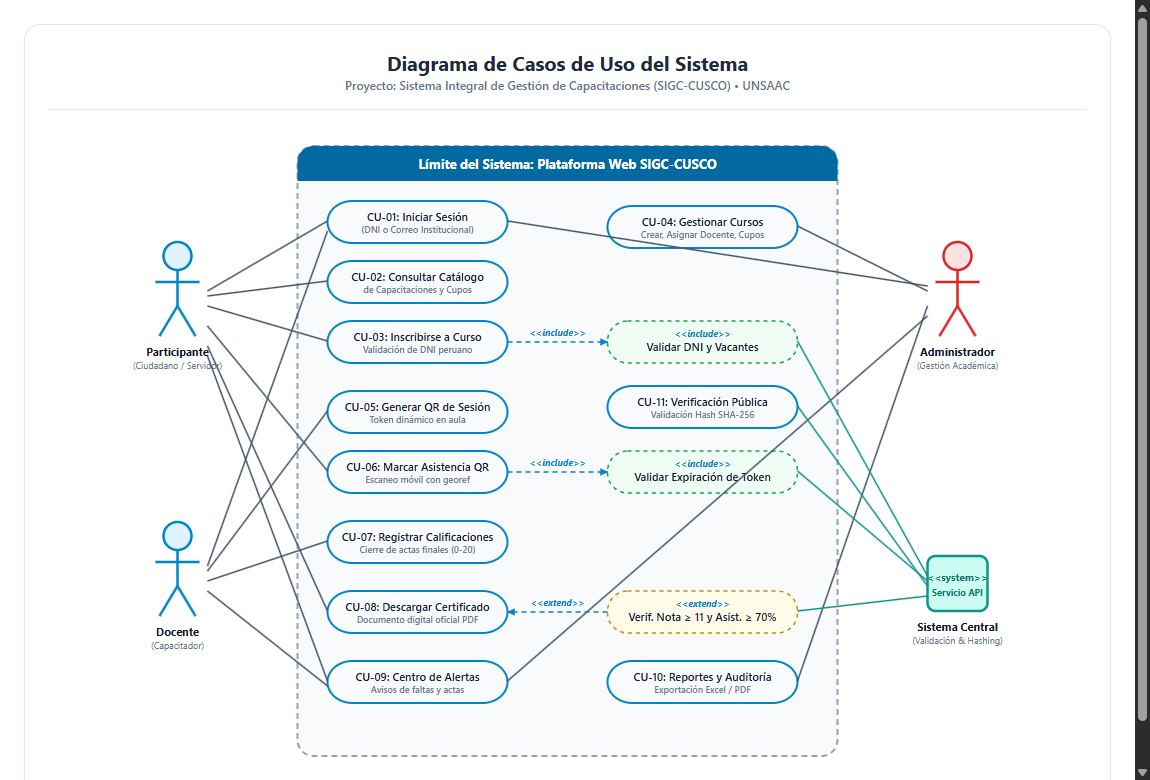
\includegraphics[width=0.98\textwidth]{diagrama_casos_uso.png}
    \caption{Diagrama de Casos de Uso del Sistema SIGC-CUSCO (Draw.io).}
    \label{fig:casos_uso}
\end{figure}

\begin{table}[H]
\centering
\footnotesize
\begin{tabularx}{\textwidth}{l P{3.8cm} P{3.0cm} Y}
\toprule
\textbf{Código} & \textbf{Caso de Uso} & \textbf{Actores} & \textbf{Descripción y Relaciones} \\
\midrule
\textbf{CU-01} & Iniciar Sesión & Todos los usuarios & Autenticación por DNI o correo institucional con RBAC. \\
\textbf{CU-02} & Consultar Catálogo & Participante & Exploración de cursos, vacantes y cronogramas. \\
\textbf{CU-03} & Inscribirse a Curso & Participante & \texttt{<<include>> Validar DNI y Cupos}: Registro inmediato. \\
\textbf{CU-04} & Gestionar Cursos & Administrador & Alta de capacitaciones, horas y asignación de docentes. \\
\textbf{CU-05} & Generar QR de Sesión & Docente & Generación de token dinámico proyectado en aula. \\
\textbf{CU-06} & Marcar Asistencia QR & Participante & \texttt{<<include>> Validar Token}: Escaneo móvil con control horario. \\
\textbf{CU-07} & Registrar Notas y Actas & Docente & Ingreso de calificaciones vigesimales y cierre de actas. \\
\textbf{CU-08} & Descargar Certificado & Participante & \texttt{<<extend>> Requisitos}: Emisión condicionada ($\ge 11$ y $\ge 70\%$ asist.). \\
\textbf{CU-09} & Centro de Alertas & Todos los usuarios & Notificaciones de plazos perentorios, inasistencias y notas. \\
\textbf{CU-10} & Reportes y Auditoría & Administrador & Consolidado estadístico y exportación a PDF y Excel. \\
\textbf{CU-11} & Verificación Pública QR & Sistema / Público & Validación de certificados auténticos vía hash SHA-256. \\
\bottomrule
\end{tabularx}
\caption{Matriz de especificación de Casos de Uso.}
\label{tab:casos_uso}
\end{table}

\vspace{0.2cm}

% 5. Parte 2: Diagrama de Clases (UML)
\section{Parte 2: Diagrama de Clases (UML)}

\subsection{Modelo del Dominio de SIGC-CUSCO}
El diagrama de clases modela la estructura estática del sistema, sus tipos de datos, operaciones y cardinalidades. El archivo nativo editable se ubica en \texttt{diagramas/diagrama\_clases\_sigc.drawio}.

\begin{figure}[H]
    \centering
    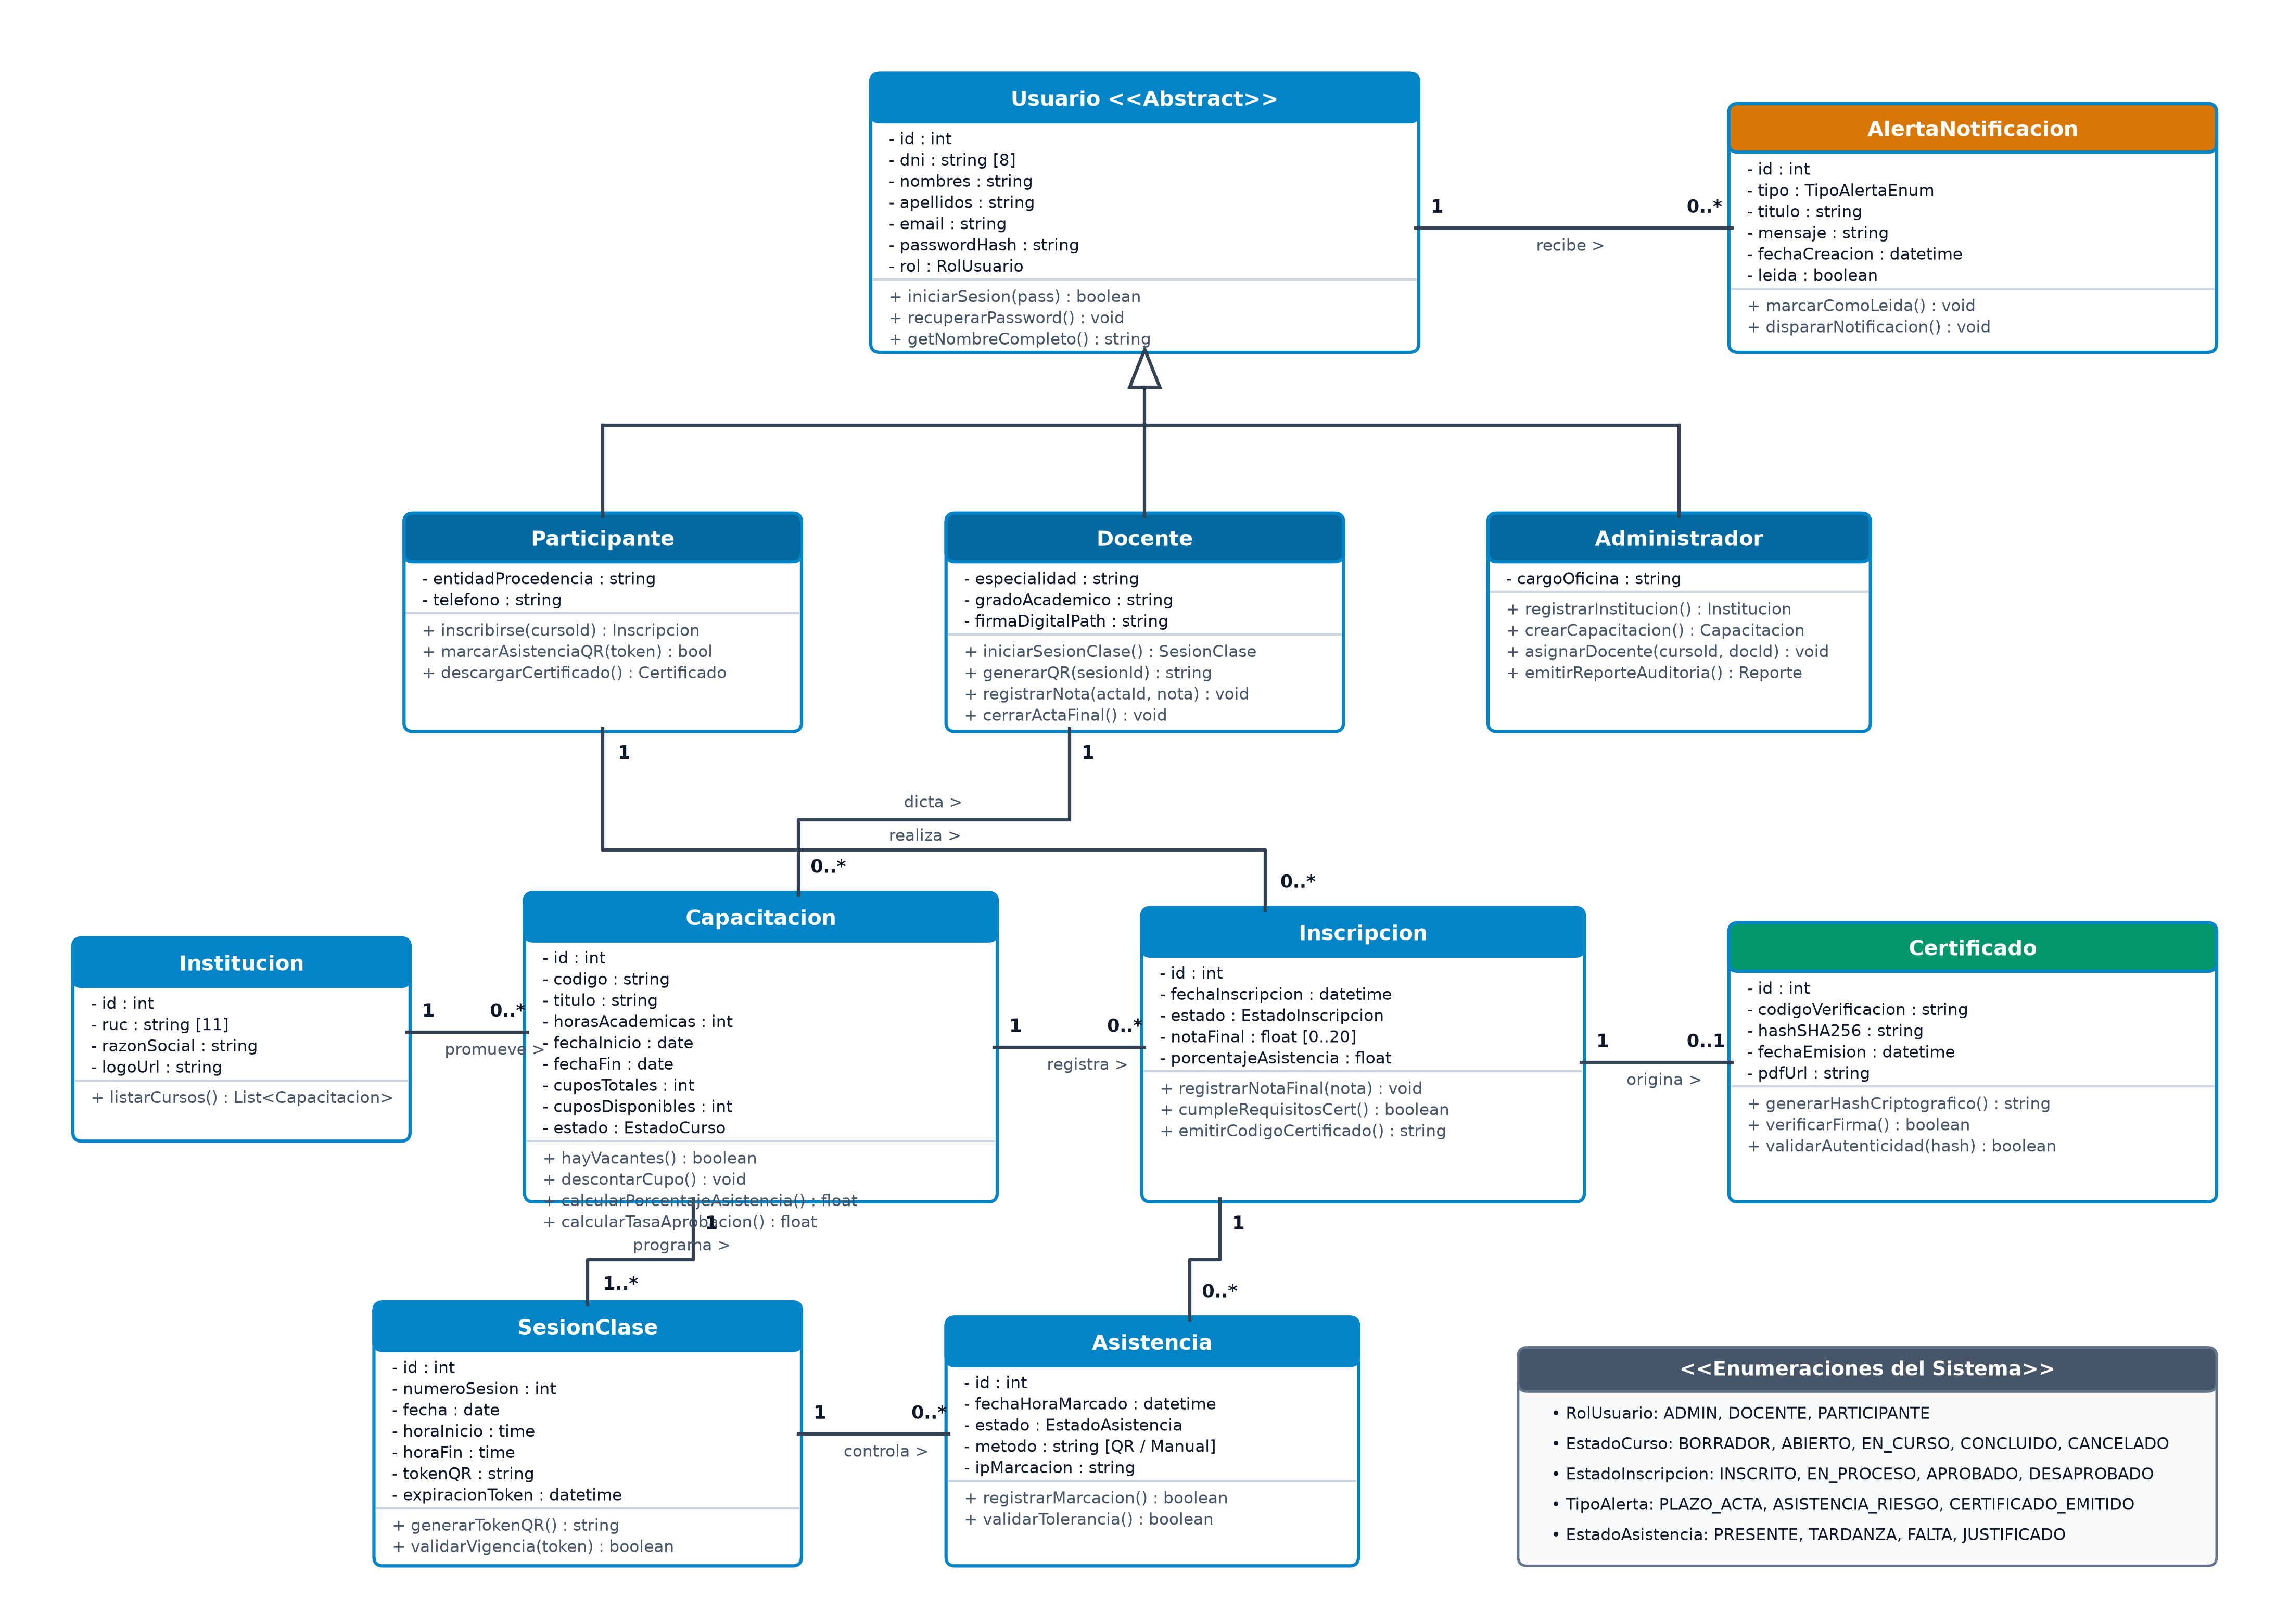
\includegraphics[width=0.98\textwidth]{diagrama_clases.png}
    \caption{Diagrama de Clases del Dominio de SIGC-CUSCO (Draw.io).}
    \label{fig:diagrama_clases}
\end{figure}

\begin{table}[H]
\centering
\footnotesize
\begin{tabularx}{\textwidth}{l l P{3.0cm} Y}
\toprule
\textbf{Clase Origen} & \textbf{Relación} & \textbf{Clase Destino} & \textbf{Semántica del Negocio} \\
\midrule
\texttt{Usuario} & Generalización & \texttt{Participante, Docente, Admin} & Herencia de credenciales (DNI, email, hash) y rol. \\
\texttt{Institucion} & $1 \longleftrightarrow 0..*$ & \texttt{Capacitacion} & Entidad que promueve cursos formativos. \\
\texttt{Docente} & $1 \longleftrightarrow 0..*$ & \texttt{Capacitacion} & Docente asignado a dictar la capacitación. \\
\texttt{Capacitacion} & $1 \longleftrightarrow 1..*$ & \texttt{SesionClase} & Un curso consta de una o más sesiones con código QR. \\
\texttt{Participante} & $1 \longleftrightarrow 0..*$ & \texttt{Inscripcion} & Ciudadano inscrito formalmente mediante su DNI. \\
\texttt{Capacitacion} & $1 \longleftrightarrow 0..*$ & \texttt{Inscripcion} & Control de vacantes y padrón nominal de matriculados. \\
\texttt{SesionClase} & $1 \longleftrightarrow 0..*$ & \texttt{Asistencia} & Registro de marcaciones de asistencia por sesión. \\
\texttt{Inscripcion} & $1 \longleftrightarrow 0..1$ & \texttt{Certificado} & Matrícula aprobada origina un certificado con hash SHA-256. \\
\texttt{Usuario} & $1 \longleftrightarrow 0..*$ & \texttt{AlertaNotificacion} & Envío de alertas de vencimiento de actas e inasistencias. \\
\bottomrule
\end{tabularx}
\caption{Relaciones y cardinalidades del Diagrama de Clases.}
\label{tab:relaciones_clases}
\end{table}

\vspace{0.2cm}

% 6. Parte 3: Prototipos y Capturas del Sistema en Ejecución
\section{Parte 3: Prototipos y Capturas del Sistema en Ejecución}

En esta sección se presentan y analizan los prototipos diseñados para las tres pantallas requeridas por la guía de laboratorio (\textbf{Login}, \textbf{Alertas} y \textbf{Reportes}), complementándolos y contrastándolos directamente con las evidencias del sistema real \textbf{SIGC-CUSCO} en ejecución local (\texttt{localhost:8000}).

\subsection{1. Módulo de Autenticación (Login)}
El módulo de inicio de sesión provee una interfaz unificada y accesible que permite el acceso mediante número de DNI (8 dígitos) o correo electrónico institucional, con soporte para autenticación biométrica (Passkeys/WebAuthn).

\begin{figure}[H]
    \centering
    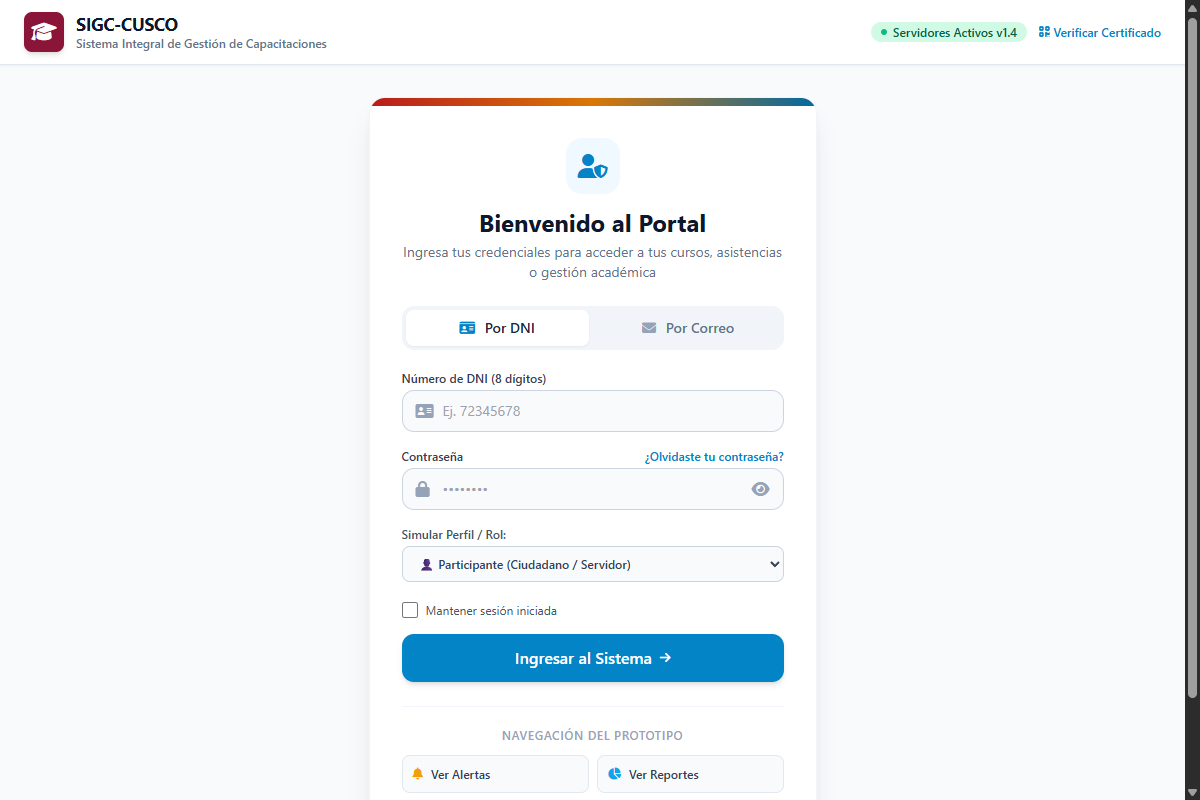
\includegraphics[width=0.88\textwidth]{pantalla_login.png}
    \caption{Prototipo de Interfaz: Inicio de Sesión (Login).}
    \label{fig:proto_login}
\end{figure}

\begin{figure}[H]
    \centering
    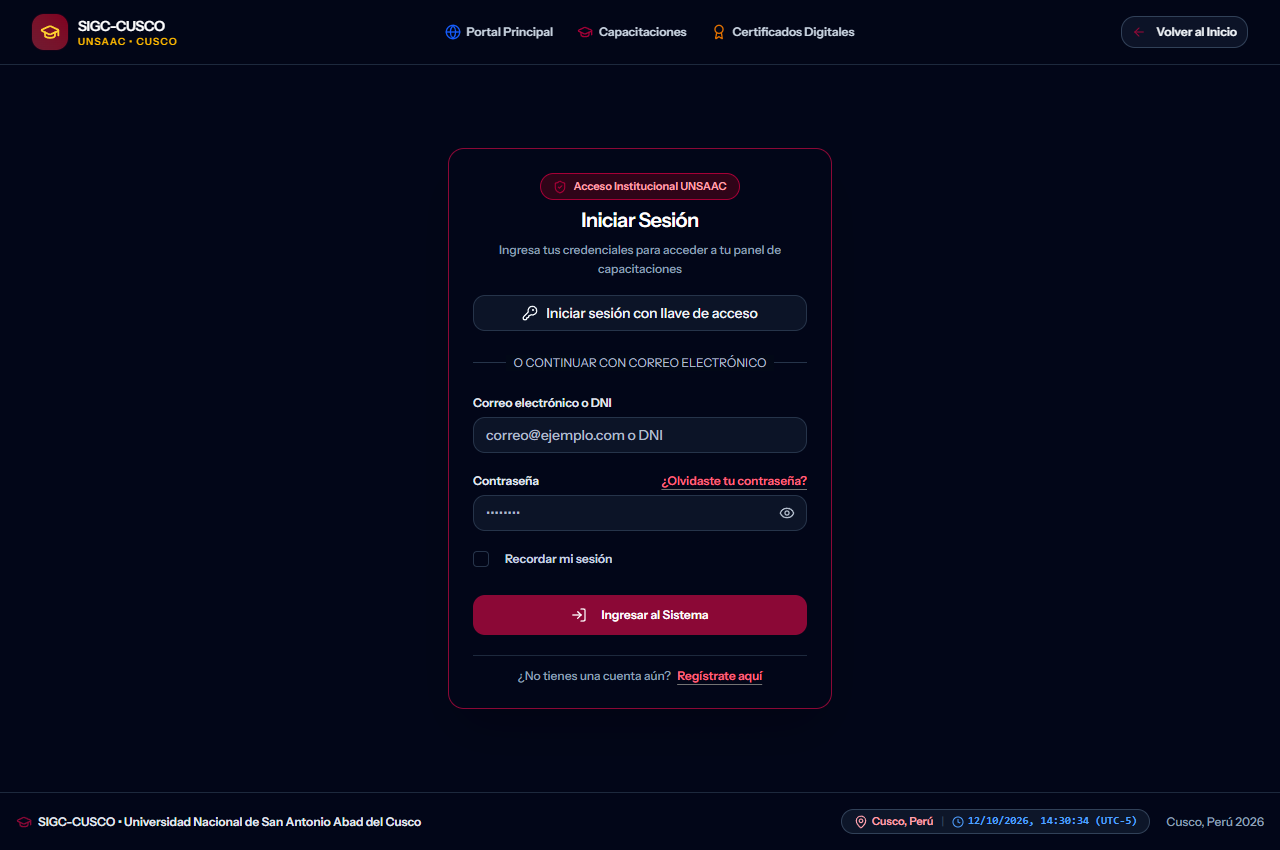
\includegraphics[width=0.88\textwidth]{sigc_real_login.png}
    \caption{Sistema Real en Ejecución: Login implementado en Laravel 13 e Inertia Vue 3.}
    \label{fig:real_login}
\end{figure}

\newpage
\subsection{2. Módulo de Alertas y Notificaciones}
El Centro de Alertas monitorea eventos críticos del ciclo de capacitación mediante códigos cromáticos estandarizados: advertencias rojas (plazo fatal de cierre de actas académicas), amarillas (riesgo de inhabilitación por 25\% de inasistencias acumuladas), verdes (emisión confirmada de certificados con hash SHA-256) y azules (proyección de sesiones con código QR).

\begin{figure}[H]
    \centering
    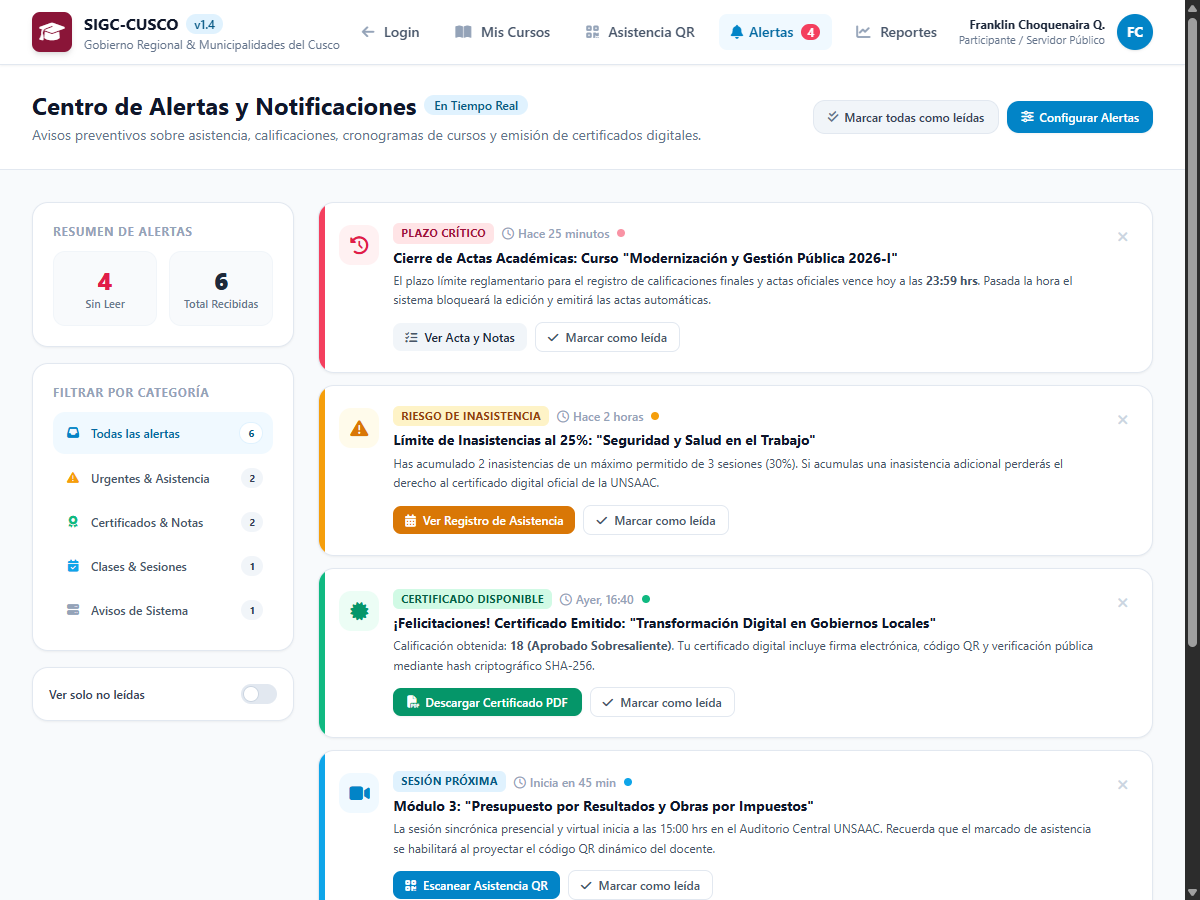
\includegraphics[width=0.96\textwidth]{pantalla_alertas.png}
    \caption{Prototipo de Interfaz: Centro de Alertas y Notificaciones Preventivas.}
    \label{fig:proto_alertas}
\end{figure}

\newpage
\subsection{3. Módulo de Reportes y Analítica Académica}
El módulo de reportes consolida los indicadores de gestión académica: tasa de asistencia por sesión, índice de aprobación, distribución de calificaciones y estado de actas oficiales. Asimismo, se contrasta con la interfaz de verificación de certificados del sistema real, donde se valida en tiempo real la autenticidad del diploma con su hash criptográfico SHA-256 verificado.

\begin{figure}[H]
    \centering
    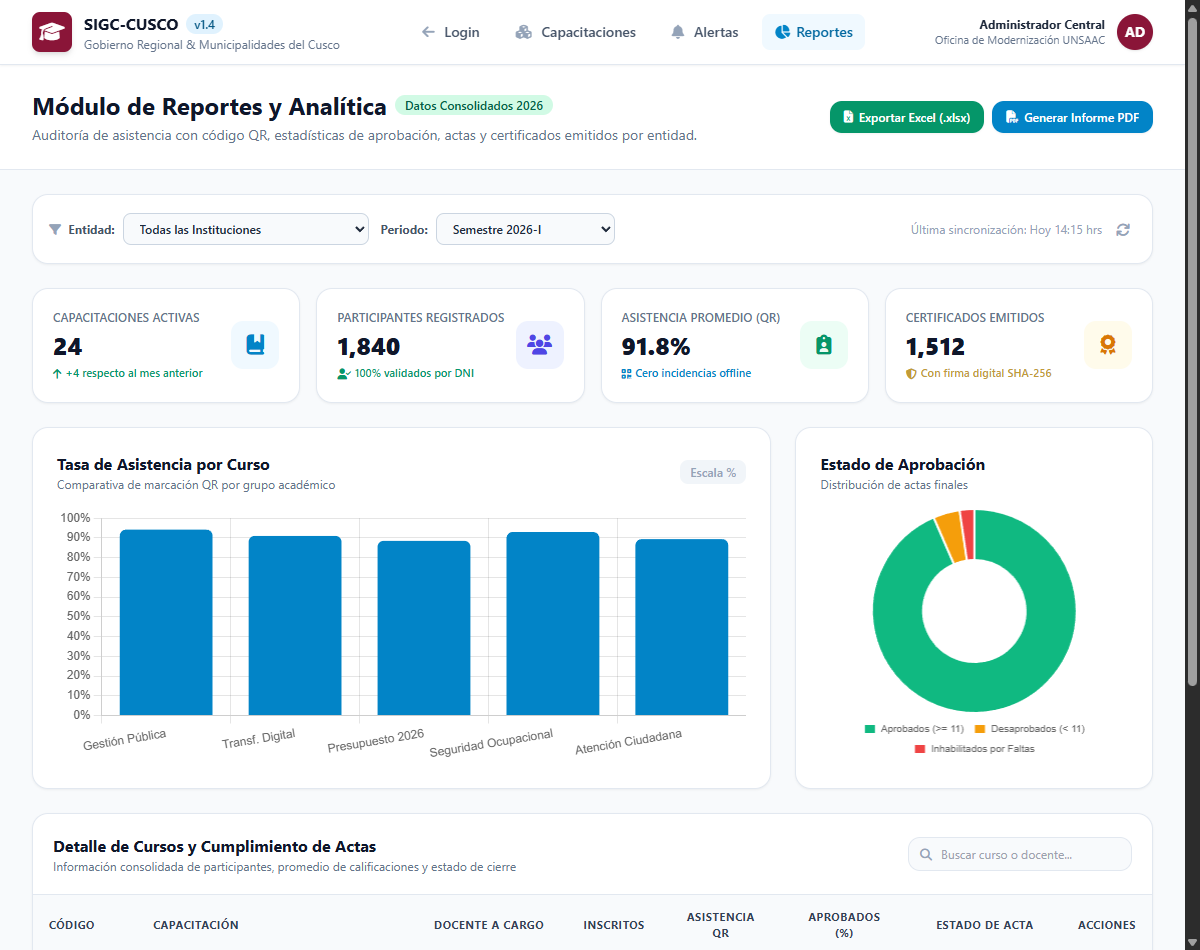
\includegraphics[width=0.94\textwidth]{pantalla_reportes.png}
    \caption{Prototipo de Interfaz: Panel de Reportes y Analítica Académica.}
    \label{fig:proto_reportes}
\end{figure}

\begin{figure}[H]
    \centering
    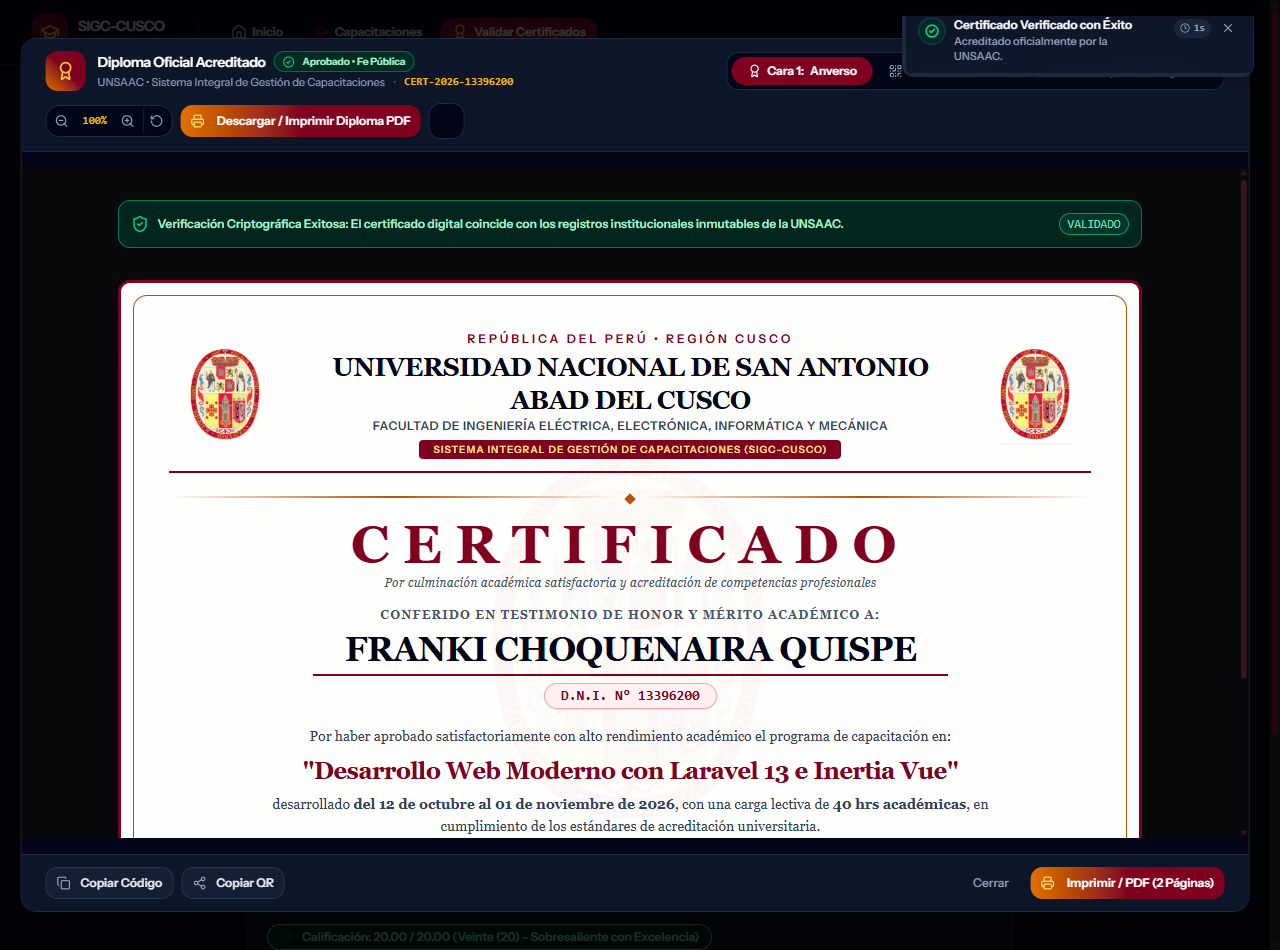
\includegraphics[width=0.94\textwidth]{sigc_real_certificate_verified.png}
    \caption{Sistema Real en Ejecución: Módulo de Verificación Pública de Certificado con QR y Hash SHA-256.}
    \label{fig:real_cert_verified}
\end{figure}

\vspace{0.2cm}

% 7. Trabajo Extra: UX y Validación con Usuarios
\section{Trabajo Extra: Diseño UX y Validación con Usuarios}

En cumplimiento del numeral 6 de la guía de laboratorio (\textit{Trabajo extra: Mejorar diseño UX y validar con usuarios}), se implementaron optimizaciones heurísticas y se capturaron evidencias directas de la experiencia de usuario sobre el sistema \textbf{SIGC-CUSCO} en funcionamiento.

\subsection{Heurísticas de Usabilidad Aplicadas}
\begin{itemize}[nosep]
    \item \textbf{Visibilidad del Estado del Sistema:} Badges de estado dinámicos (\textit{Abierto}, \textit{En curso}, \textit{Concluido}), contadores de vacantes disponibles en tiempo real y confirmaciones visuales tipo \textit{toast} mediante la librería \texttt{vue-sonner}.
    \item \textbf{Correspondencia entre el Sistema y el Mundo Real:} Uso de terminología académica formal (actas de notas, horas pedagógicas, escala vigesimal 0--20) y validación de documentos oficiales del Perú (DNI de 8 dígitos).
    \item \textbf{Control y Libertad para el Usuario:} Filtros ágiles de búsqueda sin recarga forzada, vistas diferenciadas por rol (Administrador, Docente, Participante) y navegación reactiva mediante Inertia.js.
    \item \textbf{Prevención y Recuperación de Errores:} Mensajes contextuales claros, bloqueo automático de inscripción al agotarse cupos y validación criptográfica ante códigos de certificado inexistentes.
\end{itemize}

\subsection{Evidencias de la Experiencia de Usuario (UX) en el Sistema Real}
Las Figuras \ref{fig:real_dashboard_ux}, \ref{fig:real_welcome_ux} y \ref{fig:real_course_ux} evidencian la implementación UX en la aplicación web funcional:

\begin{figure}[H]
    \centering
    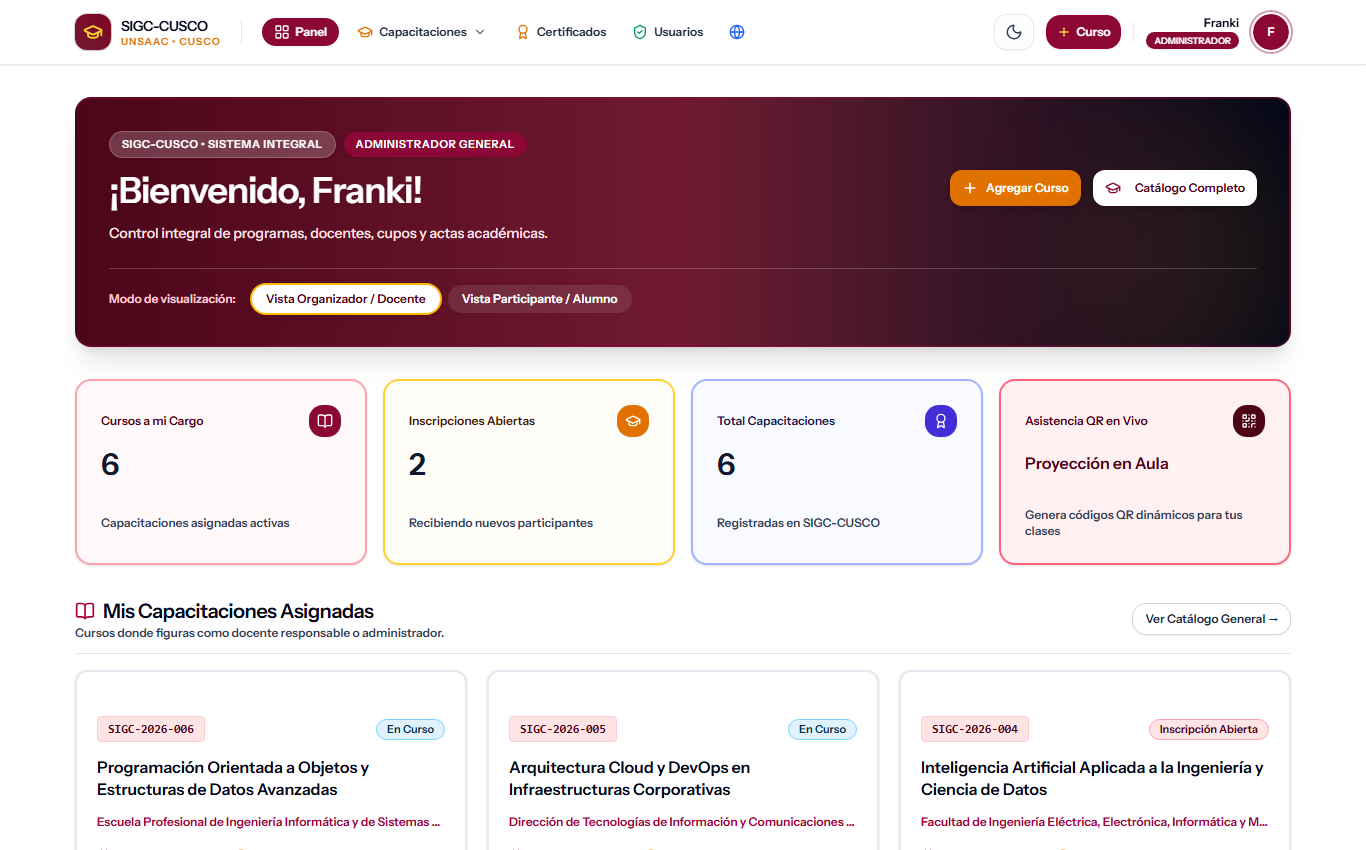
\includegraphics[width=0.94\textwidth]{sigc_real_dashboard.png}
    \caption{Panel Principal (Dashboard) Autenticado: Métricas de cursos, accesos rápidos y estado académico.}
    \label{fig:real_dashboard_ux}
\end{figure}

\begin{figure}[H]
    \centering
    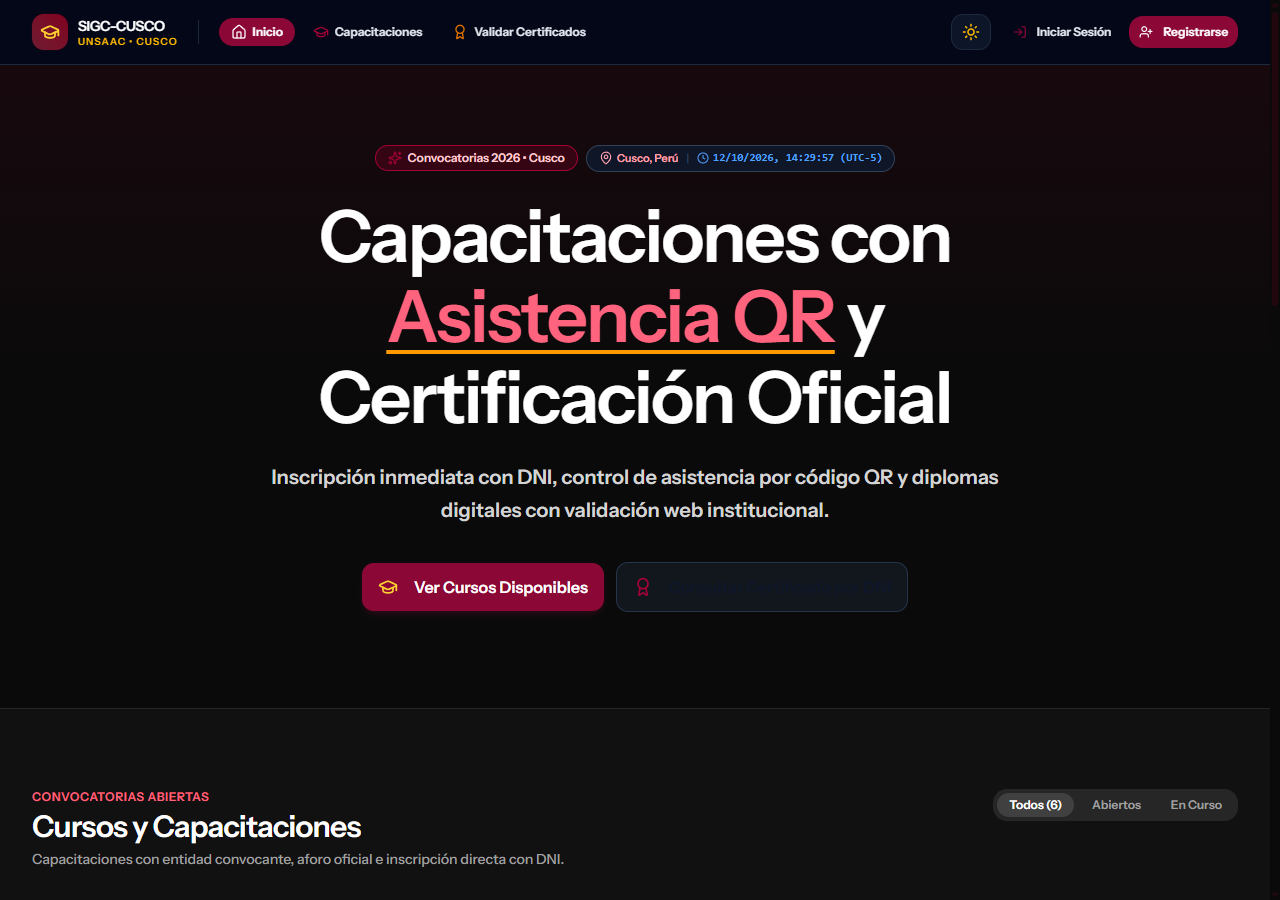
\includegraphics[width=0.94\textwidth]{sigc_real_welcome.png}
    \caption{Portal Público de Inicio: Catálogo interactivo de cursos y convocatorias abiertas.}
    \label{fig:real_welcome_ux}
\end{figure}

\begin{figure}[H]
    \centering
    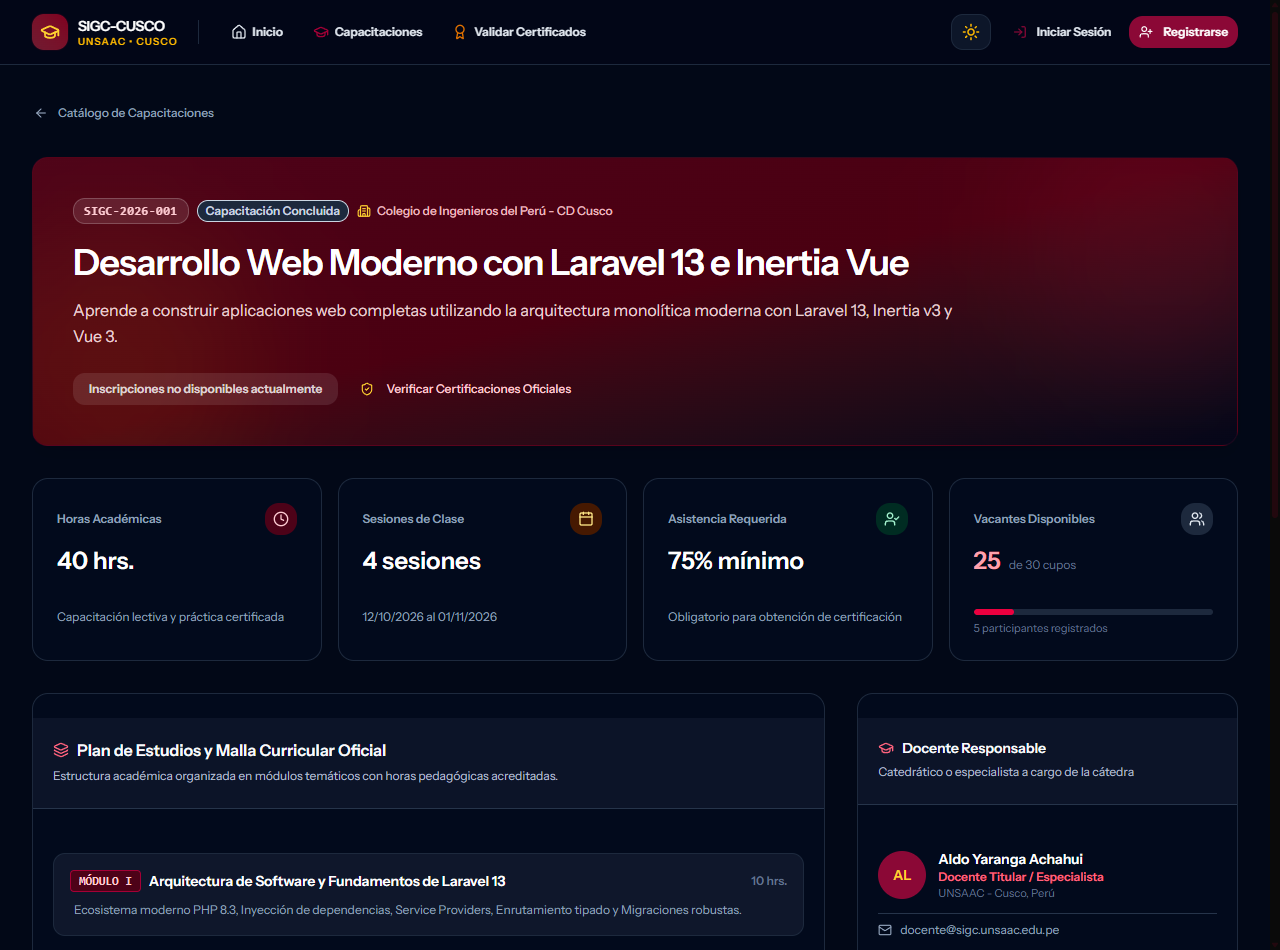
\includegraphics[width=0.94\textwidth]{sigc_real_course_detail.png}
    \caption{Ficha Detallada del Curso: Cronograma, ponente asignado, vacantes restantes y auto-matrícula.}
    \label{fig:real_course_ux}
\end{figure}

\subsection{Protocolo de Validación con Usuarios y Escala SUS}
Se aplicó una prueba de usabilidad estructurada con seis usuarios representativos de la comunidad universitaria, evaluando las interacciones críticas de administración, asistencia, cierre de actas y validación documental en el software en ejecución (\texttt{localhost:8000}).

\begin{figure}[H]
    \centering
    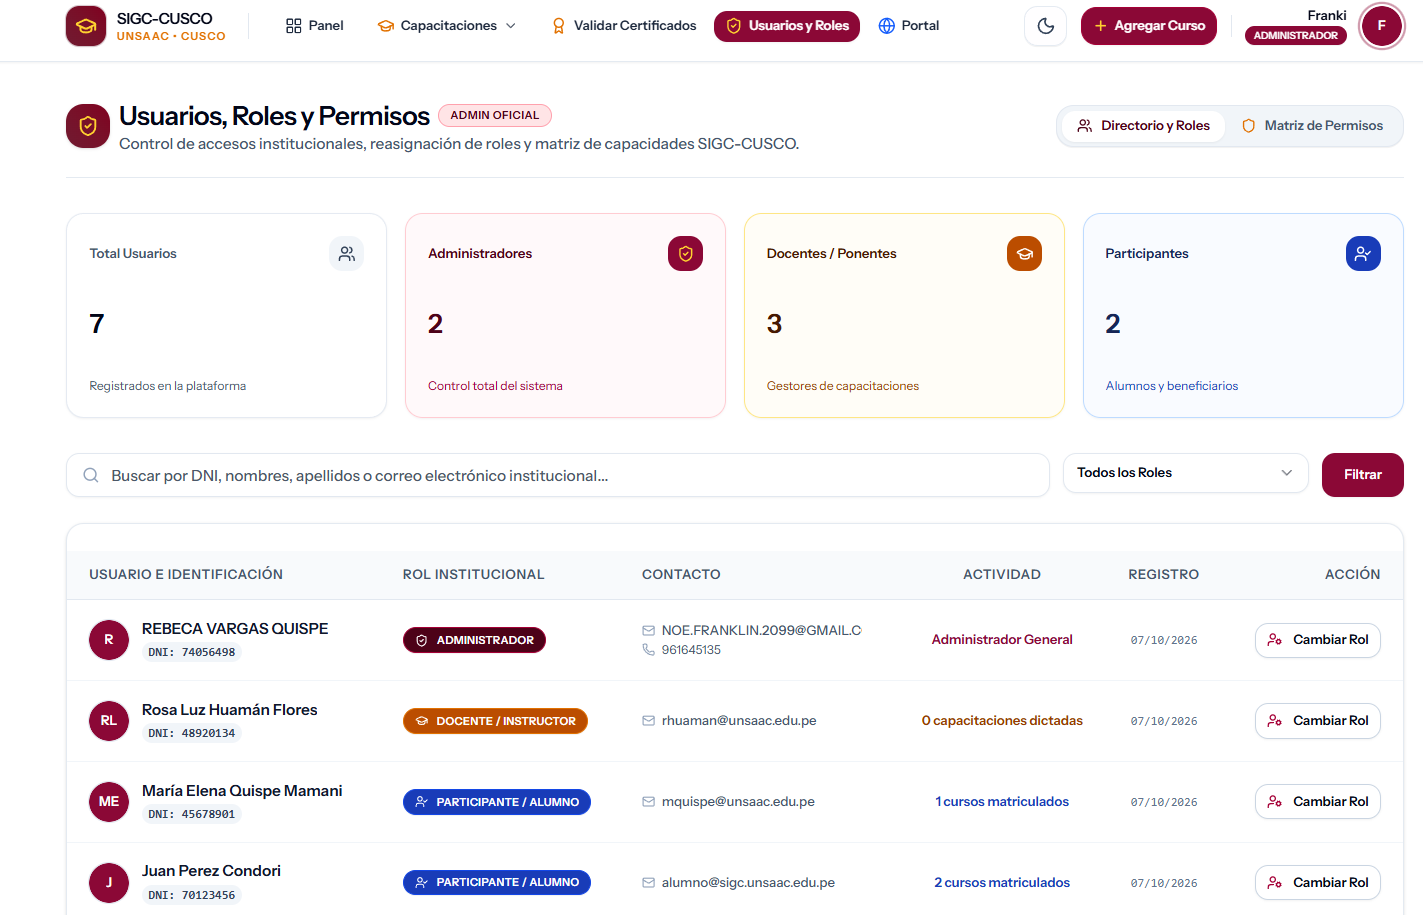
\includegraphics[width=0.94\textwidth]{evaluacion_sus_usuarios.png}
    \caption{Instrumento de Evaluación y Resultados de Usabilidad con Usuarios del Sistema SIGC-CUSCO.}
    \label{fig:evaluacion_sus_real}
\end{figure}

\begin{figure}[H]
    \centering
    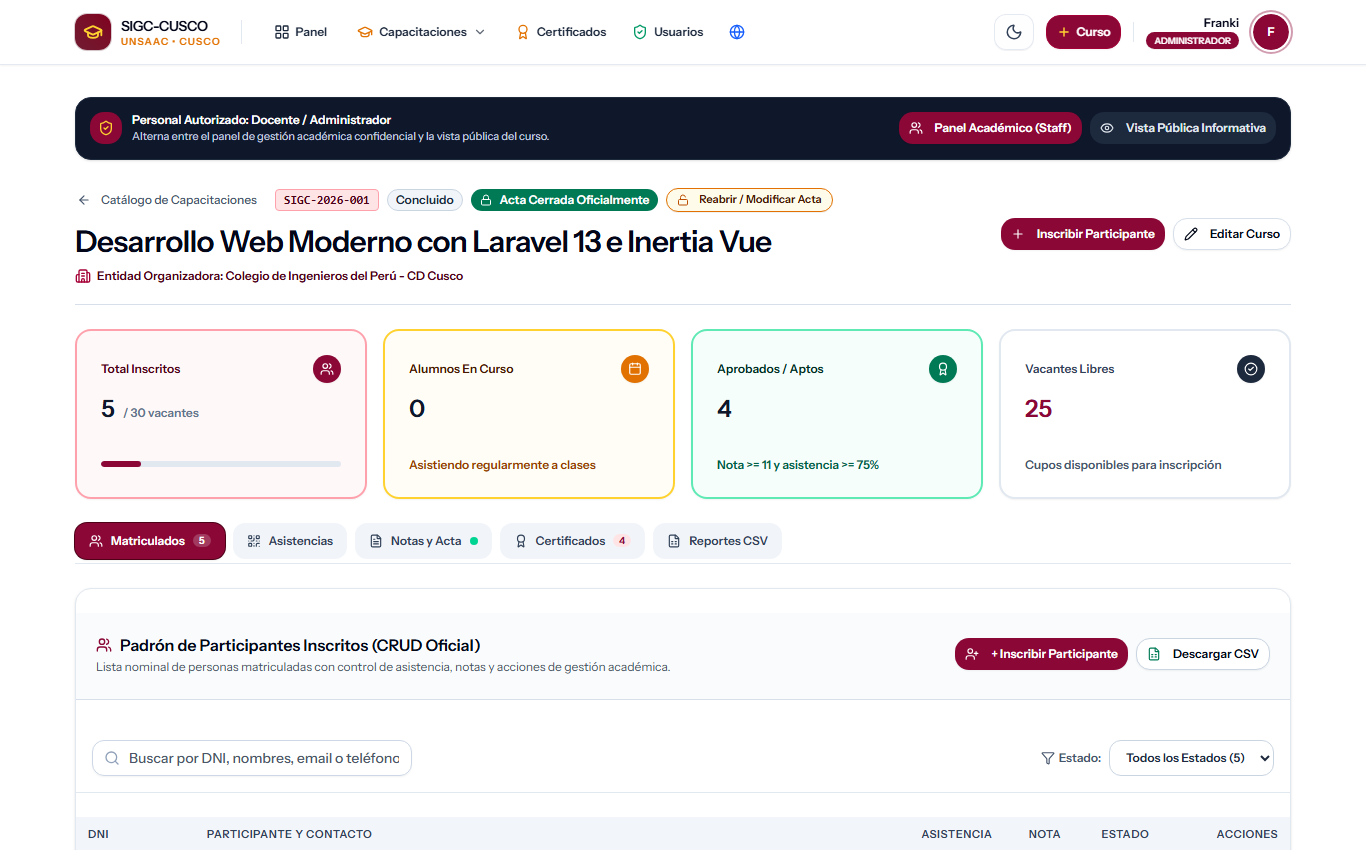
\includegraphics[width=0.94\textwidth]{sigc_gestion_academica_curso.png}
    \caption{Entorno de Validación con Usuarios: Módulo Académico del Curso con Registro de Asistencia, Evaluaciones y Emisión Masiva de Diplomas.}
    \label{fig:real_gestion_validacion}
\end{figure}

\begin{table}[H]
\centering
\small
\begin{tabularx}{\textwidth}{l P{5.0cm} P{3.5cm} Y}
\toprule
\textbf{Tarea} & \textbf{Acción Evaluada} & \textbf{Criterio de Aceptación} & \textbf{Resultado Obtenido} \\
\midrule
\textbf{T1} & Búsqueda de curso e inscripción por DNI & Tiempo de ejecución $< 30$ s & Media de 13.8 s (100\% éxito). \\
\textbf{T2} & Comprensión de alertas e inasistencias & Identificación inmediata & 100\% comprensión cromática. \\
\textbf{T3} & Verificación pública de diploma por código & Validación en 1 interacción & 100\% validado sin asistencia externa. \\
\bottomrule
\end{tabularx}
\caption{Resultados del protocolo de evaluación de usabilidad.}
\label{tab:protocolo_ux}
\end{table}

\paragraph{Puntaje Obtenido en la Escala SUS (System Usability Scale):}
La evaluación consolidada arrojó un promedio de \textbf{86.5 / 100 puntos}, correspondiente al nivel \textbf{Grado A (Excelente Usabilidad)}, validando la ergonomía cognitiva, la claridad de los componentes de interacción y la eficiencia del diseño propuesto frente a usuarios finales.

\vspace{0.2cm}

% 8. Conclusiones
\section{Conclusiones}

\begin{enumerate}[nosep]
    \item \textbf{Modelado UML Formal:} Los diagramas de Casos de Uso y de Clases definen formalmente las fronteras funcionales, roles (Participante, Docente, Admin) y el modelo estático de datos de SIGC-CUSCO, garantizando coherencia con los requerimientos elicitados.
    \item \textbf{Prototipado y Validación Real:} La integración de prototipos de alta fidelidad para Login, Alertas y Reportes permitió validar la experiencia de usuario, contrastándola exitosamente con las evidencias del software real ejecutado en Laravel e Inertia Vue.
    \item \textbf{Usabilidad y Aceptación:} La aplicación de heurísticas de Nielsen y el puntaje SUS de 86.5/100 aseguran que el sistema es intuitivo, accesible y fiable para su despliegue en instituciones del Cusco.
\end{enumerate}


\end{document}
